$  $% !TeX spellcheck = de_DE
%Die Angabe des schlauen Spruchs auf diesem Wege funtioniert nur,
%wenn keine Änderung des Kapitels mittels den in preambel/chapterheads.tex
%vorgeschlagenen Möglichkeiten durchgeführt wurde.
\setchapterpreamble[u]{%
	\dictum[Albert Einstein]{Probleme kann man niemals mit derselben Denkweise lösen, durch die sie entstanden sind.}
}
\chapter{Additional OBSW examples}
\label{chap: Extra examples}

The code generator implemented as a part of this Master thesis, is also tested with other example OBSW models, designed using the OSRA SCM Model editor. Each of these examples are carefully constructed to capture all the corner cases listed in the section \cref{section: Corner cases}. The complexity of each of these models is much higher when compared to the running simple OSRA example model.

\section{Producer consumer problem}


\section{Building block approach}
The Component based approach is one of the high level requirements discussed in the chapter \cref{chap:OSRA}. According to this requirement, it should be possible to design the software as a combination of reusable units. The reusable units, being component instances, the aim of this example to reiterate the CBSE approach by having multiple component instances which correspond to the same component type.

\begin{figure}[h]
	\centering
	\subfloat[Data types, events, exceptions and interfaces diagram]{%
		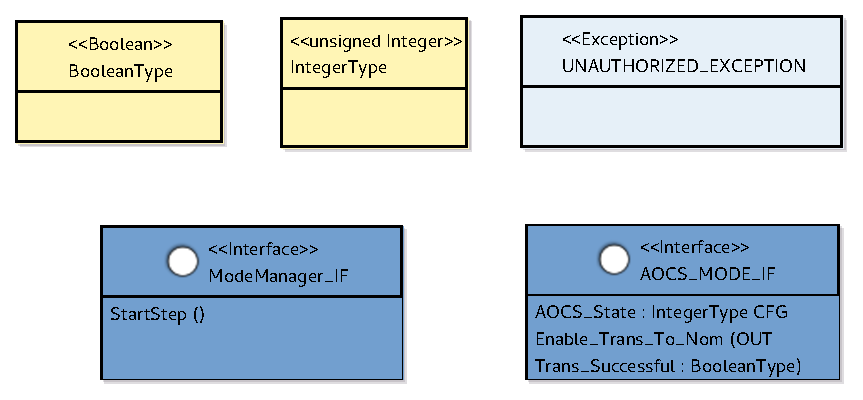
\includegraphics[width=0.8\columnwidth,keepaspectratio]{InterfacesEventsDatasetsDiagramBBA.pdf}
	}\hfill
	\subfloat[Component types diagram]{%
		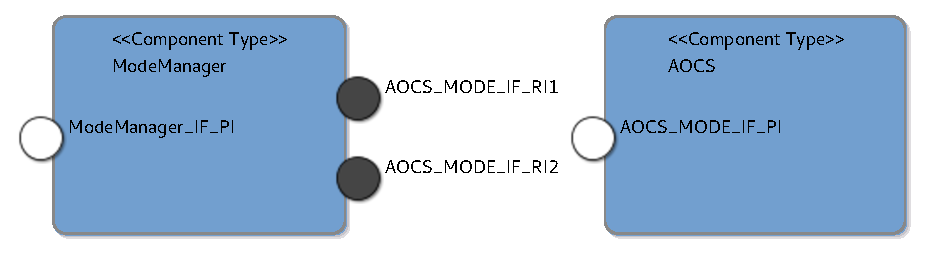
\includegraphics[width=0.8\columnwidth,keepaspectratio]{ComponentTypesDiagramBBA.pdf}
	}\hfill
	\subfloat[Component instances diagram]{%
		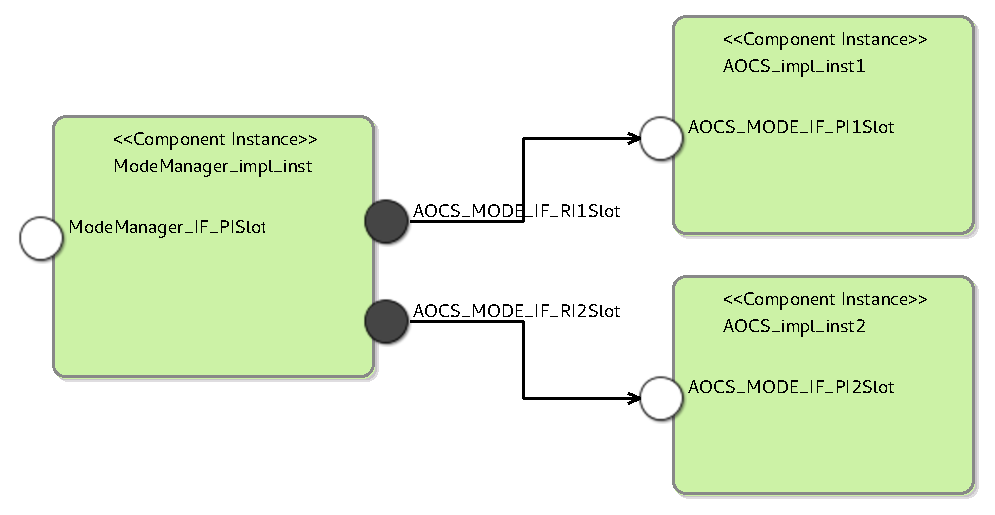
\includegraphics[width=0.8\columnwidth,keepaspectratio]{ComponentInstancesDiagramBBA.pdf}
	}%
	\caption{Building block approach example}
\end{figure}

\section{Component chaining}
As discussed before in the initial chapters, the composability and compositionality are one the corner-stone principles of the OSRA. In line with these corner-stone principles, this example aims to chain different types of components together.

\begin{figure}[h]
	\centering
	\subfloat[Data types, events, exceptions and interfaces diagram]{%
		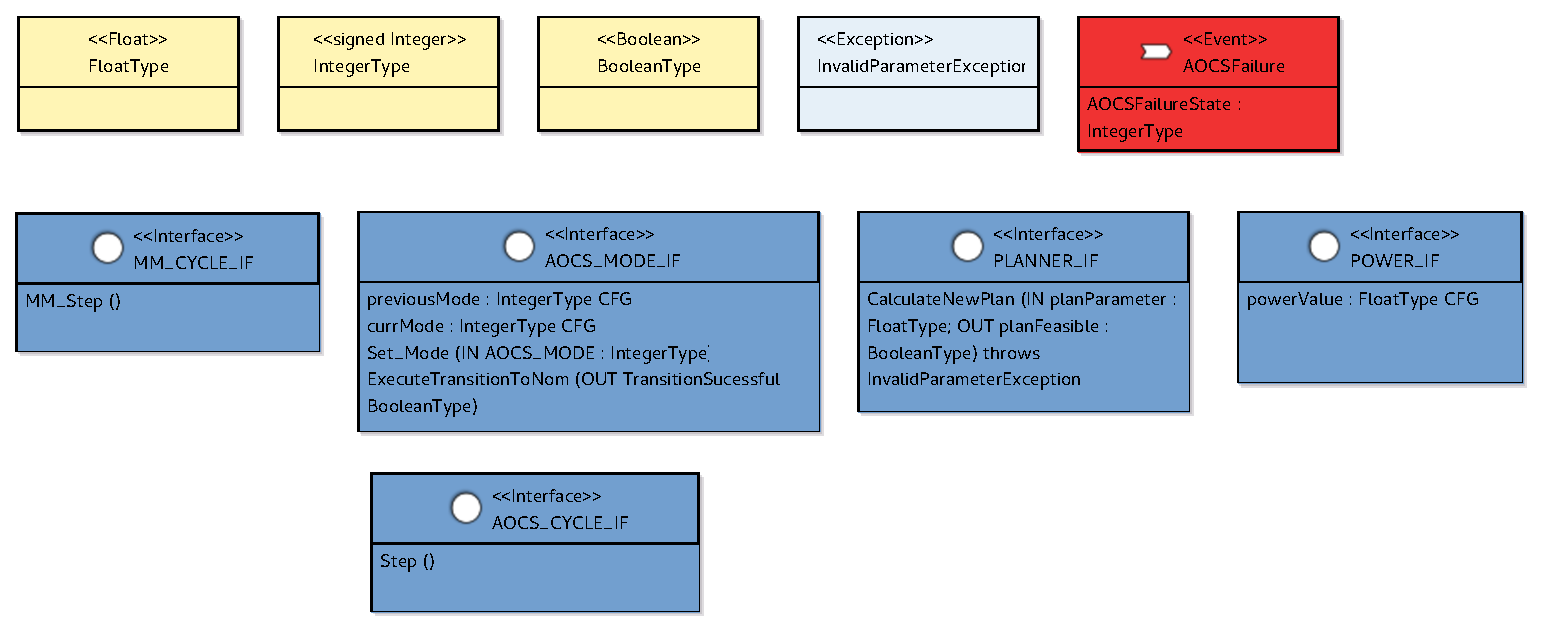
\includegraphics[width=1.0\columnwidth,keepaspectratio]{InterfacesEventsDatasetsDiagramCC.pdf}
	}\hfill
	\subfloat[Component types diagram]{%
		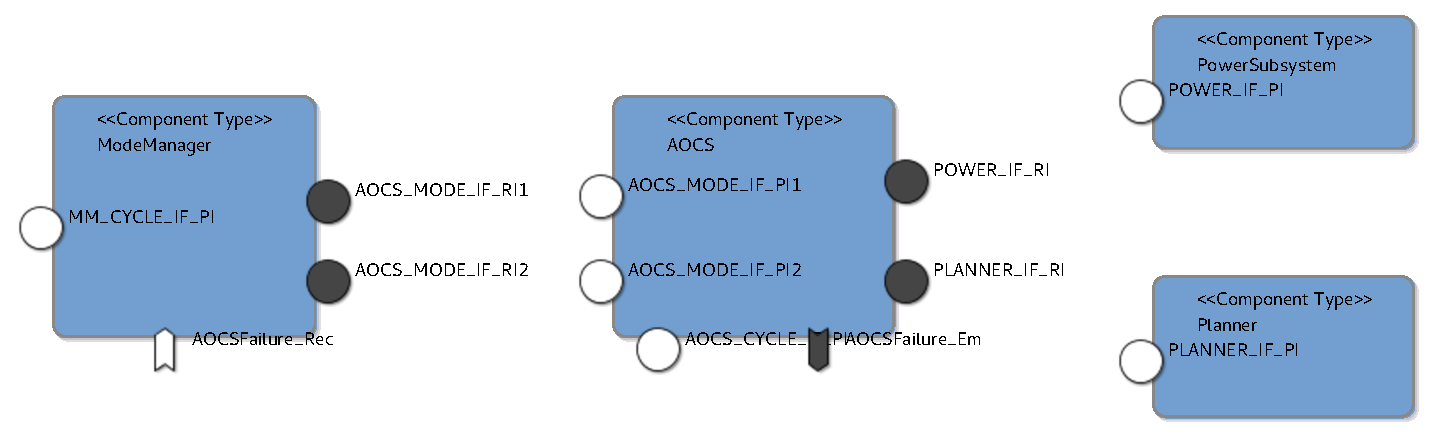
\includegraphics[width=1.0\columnwidth,keepaspectratio]{ComponentTypesDiagramCC.pdf}
	}\hfill
	\subfloat[Component instances diagram]{%
		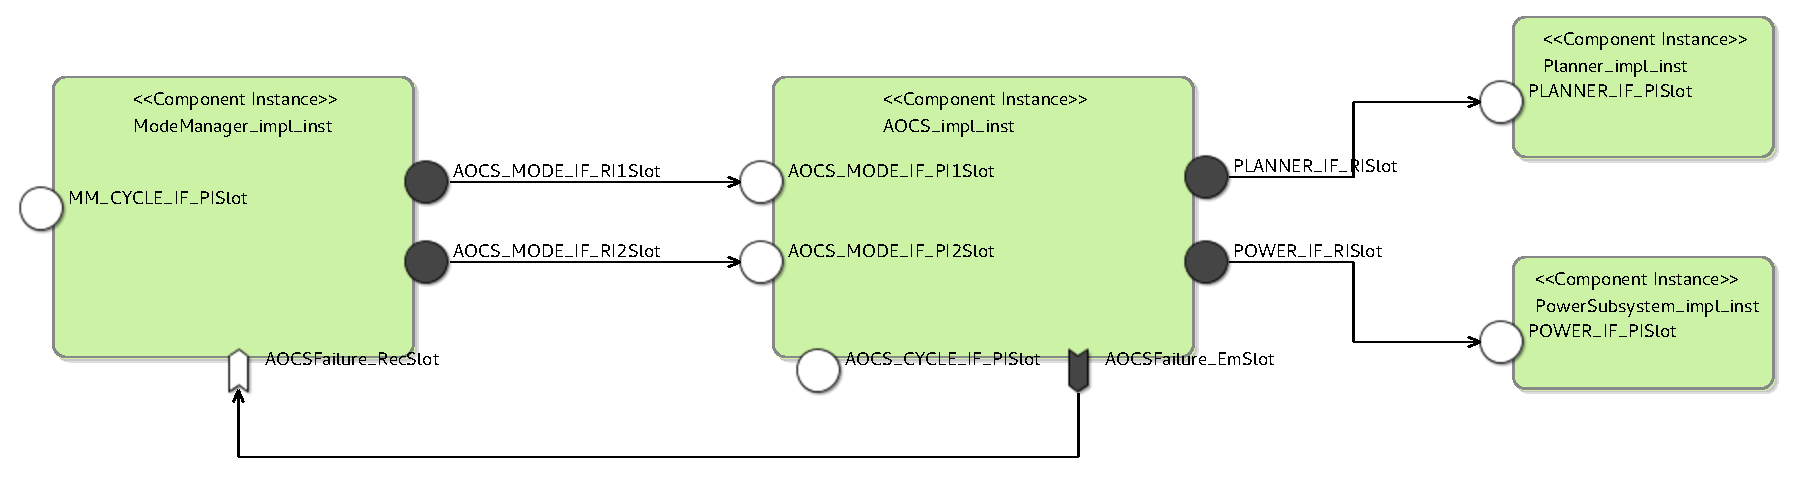
\includegraphics[width=1.0\columnwidth,keepaspectratio]{ComponentInstancesDiagramCC.pdf}
	}%
	\caption{Component chaining example}
\end{figure}

\section{Cyclic dependency}
This example 



 




   
 